%iffalse
\let\negmedspace\undefined
\let\negthickspace\undefined
\documentclass[journal,12pt,onecolumn]{IEEEtran}
\usepackage{cite}
\usepackage{amsmath,amssymb,amsfonts,amsthm}
\usepackage{algorithmic}
\usepackage{graphicx}
\usepackage{textcomp}
\usepackage{xcolor}
\usepackage{txfonts}
\usepackage{listings}
\usepackage{enumitem}
\usepackage{mathtools}
\usepackage{gensymb}
\usepackage{comment}
\usepackage[breaklinks=true]{hyperref}
\usepackage{tkz-euclide} 
\usepackage{listings}
\usepackage{gvv}
\def\inputGnumericTable{}                                 
\usepackage[latin1]{inputenc}                              
\usepackage{color}                                         
\usepackage{array}                                        
\usepackage{longtable}                                     
\usepackage{calc}                                          
\usepackage{multirow}                                      
\usepackage{hhline}                                        
\usepackage{ifthen}                                        
\usepackage{lscape}
\newtheorem{theorem}{Theorem}[section]
\newtheorem{problem}{Problem}
\newtheorem{proposition}{Proposition}[section]
\newtheorem{lemma}{Lemma}[section]
\newtheorem{corollary}[theorem]{Corollary}
\newtheorem{example}{Example}[section]
\newtheorem{definition}[problem]{Definition}
\newcommand{\BEQA}{\begin{eqnarray}}
\newcommand{\EEQA}{\end{eqnarray}}
\newcommand{\define}{\stackrel{\triangle}{=}}
\theoremstyle{remark}
\newtheorem{rem}{Remark}
\graphicspath{ {./Figures/} }
\usepackage{float} % For the [H] float option
\usepackage{textcomp}
\usepackage{multicol}

\begin{document}
\begin{enumerate}[start=1, label=Q.\arabic*]

\item If `$\rightarrow$` denotes increasing order of intensity, then the meaning of the words \brak{\text{talk $\rightarrow$ shout $\rightarrow$ scream}} is analogous to \brak{\text{please $\rightarrow$ \underline{\hspace{2cm}} $\rightarrow$ pander}}.
    Which one of the given options is appropriate to fill the blank?
    \begin{enumerate}
        \begin{multicols}{4}
        \item flatter
        \item flutter
        \item fritter
        \item frizzle
        \end{multicols}
    \end{enumerate}

    \hfill{\brak{\text{GATE EE 2024}}}

    \item P and Q have been allotted a hostel room with two beds, a study table, and an almirah. P is an avid bird-watcher and wants to sit at the table and watch birds outside the window. Q does not mind that as long as his bed is close to the ceiling fan.
    Which one of the following arrangements suits them the most?
    \begin{enumerate}
    \item
        \begin{figure}[H]
            \centering
            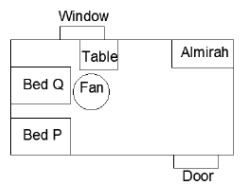
\includegraphics[width=0.4\columnwidth]{Figures/q2a.png}
        \end{figure}
    \item
        \begin{figure}[H]
            \centering
            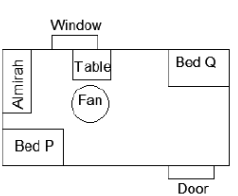
\includegraphics[width=0.4\columnwidth]{Figures/q2b.png}
        \end{figure}
    \item
        \begin{figure}[H]
            \centering
            
\includegraphics[width=0.4\columnwidth]{Figures/q2c.png}
        \end{figure}
    \item
        \begin{figure}[H]
            \centering
            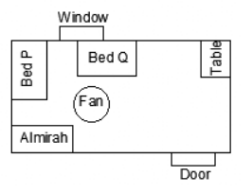
\includegraphics[width=0.4\columnwidth]{Figures/q2d.png}
        \end{figure}
    \end{enumerate}

    \hfill{\brak{\text{GATE EE 2024}}}

    \item The decimal number system uses the characters $0, 1, 2, \dots, 8, 9$, and the octal number system uses the characters $0, 1, 2, \dots, 6, 7$. For example, the decimal number $12$ \brak{=1\times10^1+2\times10^0} is expressed as $14$ \brak{=1\times8^1+4\times8^0} in the octal number system. The decimal number $108$ in the octal number system is \underline{\hspace{2cm}}.
    \begin{enumerate}
        \begin{multicols}{4}
        \item $168$
        \item $108$
        \item $150$
        \item $154$
        \end{multicols}
    \end{enumerate}

    \hfill{\brak{\text{GATE EE 2024}}}

    \item A shopkeeper buys shirts from a producer and sells them at $20\%$ profit. A customer has to pay \textsterling$3,186.00$ including $18\%$ taxes, per shirt. At what price did the shopkeeper buy each shirt from the producer?
    \begin{enumerate}
        \begin{multicols}{2}
        \item \textsterling$2,500.00$
        \item \textsterling$2,250.00$
        \item \textsterling$2,548.80$
        \item \textsterling$2,200.00$
        \end{multicols}
    \end{enumerate}

    \hfill{\brak{\text{GATE EE 2024}}}

    \item If, for non-zero real variables $x$, $y$, and real parameter $a > 1$,
    $x \colon y = \brak{a+1} \colon \brak{a-1}$,
    then, the ratio $\brak{x^2 - y^2} \colon \brak{x^2 + y^2}$ is
    \begin{enumerate}
        \begin{multicols}{2}
        \item $2a \colon \brak{a^2 + 1}$
        \item $a \colon \brak{a^2 + 1}$
        \item $2a \colon \brak{a^2 - 1}$
        \item $a \colon \brak{a^2 - 1}$
        \end{multicols}
    \end{enumerate}

    \hfill{\brak{\text{GATE EE 2024}}}

    \item In the given text, the blanks are numbered \brak{i}-\brak{iv}. Select the best match for all the blanks.
    Following a row \underline{\hspace{1cm}} \brak{i} the shopkeeper \underline{\hspace{1cm}} \brak{ii} the price of a frying pan, the cook stood \underline{\hspace{1cm}} \brak{iii} a row to withdraw cash \underline{\hspace{1cm}} \brak{iv} the ATM booth.
    \begin{enumerate}
        \item \brak{i} with \brak{ii} over \brak{iii} at \brak{iv} with
        \item \brak{i} at \brak{ii} over \brak{iii} over \brak{iv} in
        \item \brak{i} with \brak{ii} over \brak{iii} in \brak{iv} at
        \item \brak{i} over \brak{ii} with \brak{iii} over \brak{iv} at
    \end{enumerate}

    \hfill{\brak{\text{GATE EE 2024}}}

    \item In the following figure, $CD = 5$ cm, $BE = 10$ cm, $AE = 12$ cm, $\angle DAB = \angle DCB$, and $\angle DAE = \angle DBC = 90\degree$. Points AFCD create a rhombus.
    \begin{figure}[H]
        \centering
        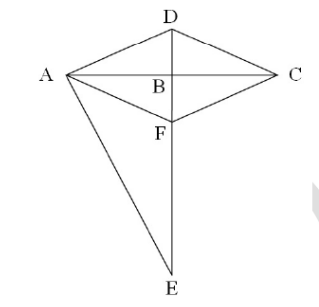
\includegraphics[width=0.3\columnwidth]{Figures/q7.png}
        \caption*{}
    \end{figure}
    The length of BF \brak{in cm} is
    \begin{enumerate}
        \begin{multicols}{4}
        \item $3$
        \item $2$
        \item $4$
        \item $6$
        \end{multicols}
    \end{enumerate}

    \hfill{\brak{\text{GATE EE 2024}}}

    \item The chart below shows the data of the number of cars bought by Millennials and Gen X people in a country from the year $2010$ to $2020$ as well as the yearly fuel consumption of the country \brak{in Million liters}.
    \begin{figure}[H]
        \centering
        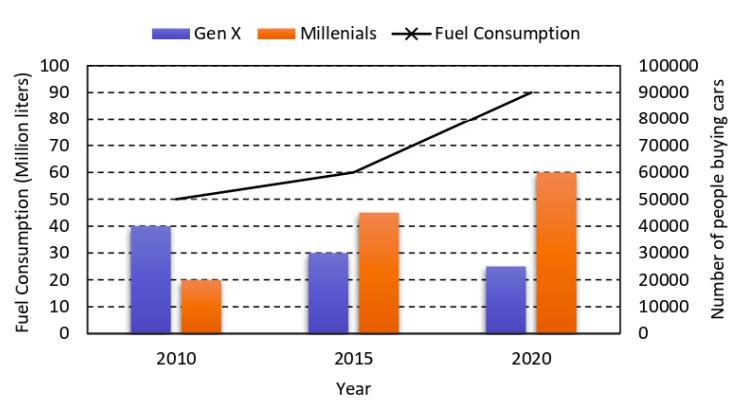
\includegraphics[width=0.8\columnwidth]{Figures/q8.png}
        \caption*{}
    \end{figure}
    Considering the data presented in the chart, which one of the following options is true?
    \begin{enumerate}
        \item The percentage increase in fuel consumption from $2010$ to $2015$ is more than the percentage increase in fuel consumption from $2015$ to $2020$.
        \item The increase in the number of Millennial car buyers from $2015$ to $2020$ is less than the decrease in the number of Gen X car buyers from $2010$ to $2015$.
        \item The increase in the number of Millennial car buyers from $2010$ to $2015$ is more than the decrease in the number of Gen X car buyers from $2010$ to $2015$.
        \item The decrease in the number of Gen X car buyers from $2015$ to $2020$ is more than the increase in the number of Millennial car buyers from $2010$ to $2015$.
    \end{enumerate}

    \hfill{\brak{\text{GATE EE 2024}}}
\item The assembly shown below has three teethed circular objects \brak{\text{Pinions}} and two teethed flat objects \brak{\text{Racks}}, which are perfectly mating with each other. Pinions can only rotate clockwise or anti-clockwise staying at its own center. Racks can translate towards the left \brak{\leftarrow} or the right \brak{\rightarrow} direction.
    \begin{figure}[H]
        \centering
        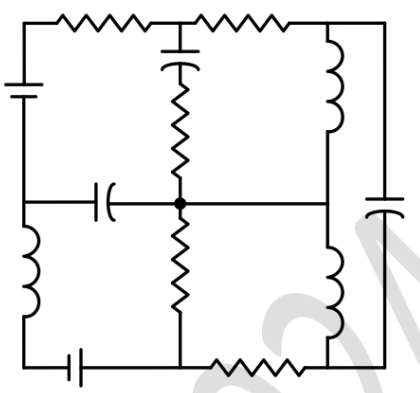
\includegraphics[width=0.5\columnwidth]{Figures/q12.png}
        \caption*{}
    \end{figure}
    If the object A \brak{\text{Rack}} is translating towards the right \brak{\rightarrow} direction, the correct statement among the following is

    \begin{enumerate}
        \item Object B translates towards the right direction.
        \item Object B translates towards the left direction.
        \item Object R rotates in the anticlockwise direction.
        \item Object Q rotates in the clockwise direction.
    \end{enumerate}

    \hfill{\brak{\text{GATE EE 2024}}}

    \item A surveyor has to measure the horizontal distance from her position to a distant reference point C. Using her position as the center, a $200$ m horizontal line segment is drawn with the two endpoints A and B. Points A, B, and C are not collinear. Each of the angles $\angle CAB$ and $\angle CBA$ are measured as $87.8\degree$. The distance \brak{in m} of the reference point C from her position is nearest to
    \begin{enumerate}
        \begin{multicols}{4}
        \item $2603$
        \item $2606$
        \item $2306$
        \item $2063$
        \end{multicols}
    \end{enumerate}

    \hfill{\brak{\text{GATE EE 2024}}}


    \item Which one of the following matrices has an inverse?
    \begin{enumerate}
        \item $\myvec{1 & 4 & 8 \\ 0 & 4 & 2 \\ 0.5 & 2 & 4}$
        \item $\myvec{1 & 2 & 3 \\ 2 & 4 & 6 \\ 3 & 2 & 9}$
        \item $\myvec{1 & 4 & 8 \\ 0 & 4 & 2 \\ 1 & 2 & 4}$
        \item $\myvec{1 & 4 & 8 \\ 0 & 4 & 2 \\ 3 & 12 & 24}$
    \end{enumerate}

    \hfill{\brak{\text{GATE EEYEAR}}}

    \item The number of junctions in the circuit is
    \begin{figure}[H]
        \centering
        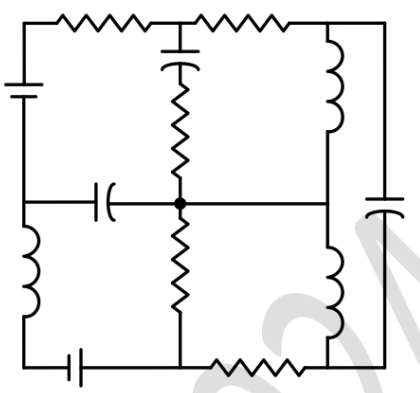
\includegraphics[width=0.5\columnwidth]{Figures/q12.png}
        \caption{}
    \end{figure}
    \begin{enumerate}
        \begin{multicols}{4}
            \item $6$
            \item $7$
            \item $8$
            \item $9$
        \end{multicols}
    \end{enumerate}

    \hfill{\brak{\text{GATE EE 2024}}}

    \item All the elements in the circuit are ideal. The power delivered by the $10$ V source in watts is
    \begin{figure}[H]
        \centering
        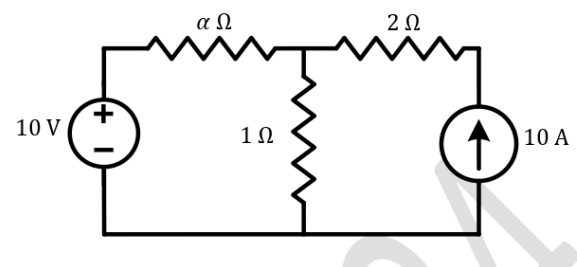
\includegraphics[width=0.5\columnwidth]{Figures/q13.png}
        \caption{}
    \end{figure}
    \begin{enumerate}
        \item $0$
        \item $50$
        \item $100$
        \item dependent on the value of $\alpha$
    \end{enumerate}

    \hfill{\brak{\text{GATE EE 2024}}}

\item The circuit shown in the figure with the switch $S$ open, is in steady state. After switch $S$ is closed, the time constant of the circuit in seconds is
    \begin{figure}[H]
        \centering
        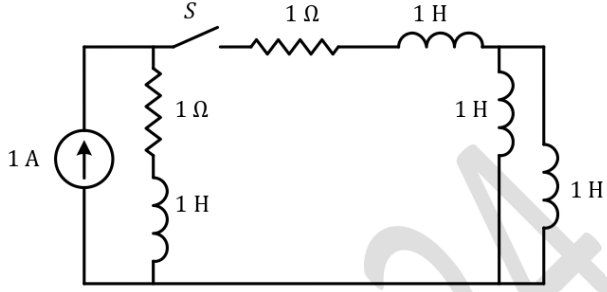
\includegraphics[width=0.5\columnwidth]{Figures/q14.png}
        \caption{}
    \end{figure}
    \begin{enumerate}
        \item $1.25$
        \item $0$
        \item $1$
        \item $1.5$
    \end{enumerate}

    \hfill{\brak{\text{GATE EE 2024}}}

    \item Suppose signal $y\brak{t}$ is obtained by the time-reversal of signal $x\brak{t}$, i.e., $y\brak{t} = x\brak{-t}$, $-\infty < t < \infty$. Which one of the following options is always true for the convolution of $x\brak{t}$ and $y\brak{t}$?
    \begin{enumerate}
        \item It is an even signal.
        \item It is an odd signal.
        \item It is a causal signal.
        \item It is an anti-causal signal.
    \end{enumerate}

    \hfill{\brak{\text{GATE EE 2024}}}
\item If $u\brak{t}$ is the unit step function, then the region of convergence \brak{ROC} of the Laplace transform of the signal $x\brak{t} = e^{5t}\brak{u\brak{t-1} - u\brak{t-10}}$ is
    \begin{enumerate}
        \item $-\infty < \text{Re}\brak{s} < \infty$
        \item $\text{Re}\brak{s} \ge 10$
        \item $\text{Re}\brak{s} \le 1$
        \item $1 \le \text{Re}\brak{s} \le 10$
    \end{enumerate}

    \hfill{\brak{\text{GATE EE 2024}}}

    \item A three phase, $50$ Hz, $6$ pole induction motor runs at $960$ rpm. The stator copper loss, core loss, and the rotational loss of the motor can be neglected. The percentage efficiency of the motor is \underline{\hspace{2cm}}.
    \begin{enumerate}
        \begin{multicols}{4}
            \item $92$
            \item $94$
            \item $96$
            \item $98$
        \end{multicols}
    \end{enumerate}

    \hfill{\brak{\text{GATE EE 2024}}}

    \item Which one of the following options represents possible voltage polarities in a single phase two winding transformer? Here, $V_p$ is the applied primary voltage, $E_p$ is the induced primary voltage, $V_s$ is the open circuit secondary voltage, and $E_s$ is the induced secondary voltage.
    \begin{enumerate}
        \item \begin{figure}[H]
        \centering
        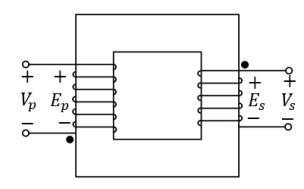
\includegraphics[width=0.4\columnwidth]{Figures/q18a.png}
        \caption{}
    \end{figure}
    \item \begin{figure}[H]
        \centering
        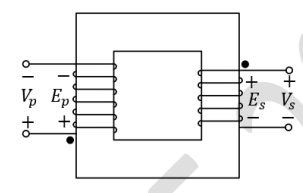
\includegraphics[width=0.4\columnwidth]{Figures/q18b.png}
        \caption{}
    \end{figure}
    \item \begin{figure}[H]
        \centering
        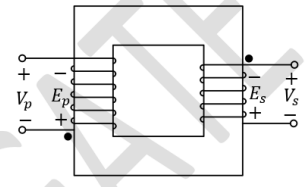
\includegraphics[width=0.4\columnwidth]{Figures/q18c.png}
        \caption{}
    \end{figure}
    \item \begin{figure}[H]
        \centering
        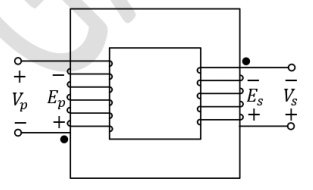
\includegraphics[width=0.4\columnwidth]{Figures/q18d.png}
        \caption{}
    \end{figure}
    \end{enumerate}

    \hfill{\brak{\text{GATE EE 2024}}}
\item The figure shows the single line diagram of a $4$-bus power network. Branches $b_1, b_2, b_3,$ and $b_4$ have impedances $4z, z, 2z,$ and $4z$ per-unit \brak{pu}, respectively, where $z = r + jx$, with $r > 0$ and $x > 0$. The current drawn from each load bus \brak{marked as arrows} is equal to $I$ pu, where $I \neq 0$. If the network is to operate with minimum loss, the branch that should be opened is
    \begin{figure}[H]
        \centering
        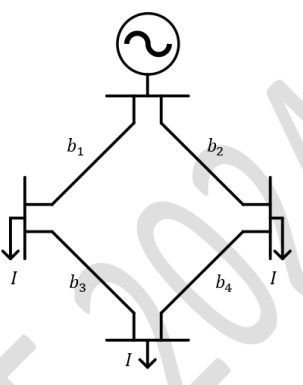
\includegraphics[width=0.5\columnwidth]{Figures/q19.png}
        \caption{}
    \end{figure}
    \begin{enumerate}
        \begin{multicols}{4}
            \item $b_1$
            \item $b_2$
            \item $b_3$
            \item $b_4$
        \end{multicols}
    \end{enumerate}

    \hfill{\brak{\text{GATE EE 2024}}}

    \item For the block-diagram shown in the figure, the transfer function $\frac{C\brak{s}}{R\brak{s}}$ is
    \begin{figure}[H]
        \centering
        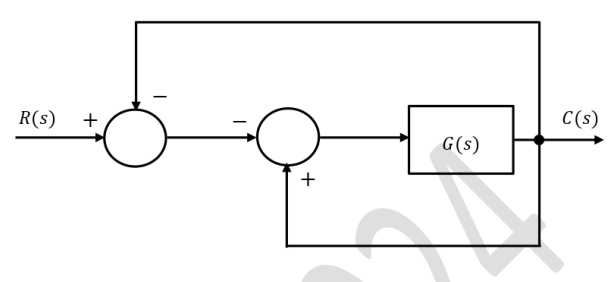
\includegraphics[width=0.5\columnwidth]{Figures/q20.png}
        \caption{}
    \end{figure}
    \begin{enumerate}
        \item $\frac{G\brak{s}}{1+2G\brak{s}}$
        \item $\frac{G\brak{s}}{1+2G\brak{s}}$
        \item $\frac{G\brak{s}}{1-2G\brak{s}}$
        \item $\frac{G\brak{s}}{1-2G\brak{s}}$
    \end{enumerate}

    \hfill{\brak{\text{GATE EE 2024}}}

    \item Consider the standard second-order system of the form $\frac{\omega_n^2}{s^2+2\zeta\omega_n s+\omega_n^2}$ with the poles $p_1$ and $p_1^*$ having negative real parts. The pole locations are also shown in the figure. Now consider two such second-order systems as defined below:
    System 1: $\omega_n = 3$ rad/sec and $\theta = 60\degree$
    System 2: $\omega_n = 1$ rad/sec and $\theta = 70\degree$
    Which one of the following statements is correct?
    \begin{figure}[H]
        \centering
        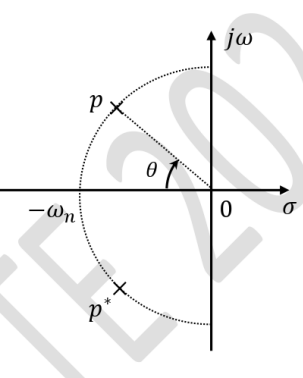
\includegraphics[width=0.4\columnwidth]{Figures/q21.png}
        \caption{}
    \end{figure}
    \begin{enumerate}
        \item Settling time of System 1 is more than that of System 2.
        \item Settling time of System 2 is more than that of System 1.
        \item Settling times of both the systems are the same.
        \item Settling time cannot be computed from the given information.
    \end{enumerate}

    \hfill{\brak{\text{GATE EE 2024}}}

    \item Consider the cascaded system as shown in the figure. Neglecting the faster component of the transient response, which one of the following options is a first order pole-only approximation such that the steady-state values of the unit step responses of the original and the approximated systems are same?
    \begin{figure}[H]
        \centering
        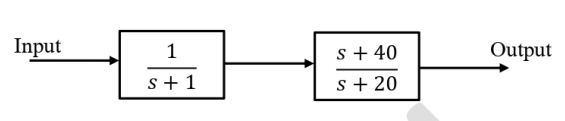
\includegraphics[width=0.6\columnwidth]{Figures/q22.png}
        \caption{}
    \end{figure}
    \begin{enumerate}
        \begin{multicols}{2}
            \item $\frac{1}{s+1}$
            \item $\frac{2}{s+1}$
            \item $\frac{1}{s+20}$
            \item $\frac{2}{s+20}$
        \end{multicols}
    \end{enumerate}

    \hfill{\brak{\text{GATE EE 2024}}}

    \item The table lists two instrument transformers and their features:
    \begin{table}[H]
        \centering
        \begin{tabular}{|l|l|}
            \hline
            \textbf{Instrument Transformers} & \textbf{Features} \\
            \hline
            X) Current Transformer \brak{CT} & P) Primary is connected in parallel to the grid \\
            Y) Potential Transformer \brak{PT} & Q) Open circuited secondary is not desirable \\
            & R) Primary current is the line current \\
            & S) Secondary burden affects the primary current \\
            \hline
        \end{tabular}
        \caption*{}
        \label{tab:q23}
    \end{table}
    The correct matching of the two columns is
    \begin{enumerate}
        \item X matches with P and Q; Y matches with R and S.
        \item X matches with P and R; Y matches with Q and S.
        \item X matches with Q and R; Y matches with P and S.
        \item X matches with Q and S; Y matches with P and R.
    \end{enumerate}

    \hfill{\brak{\text{GATE EE 2024}}}

    \item Simplified form of the Boolean function $F\brak{P,Q,R,S} = PQ + \overline{P}QS + \overline{P}\overline{Q}RS + \overline{P}\overline{Q}\overline{R}S$ is
    \begin{enumerate}
        \begin{multicols}{2}
            \item $PS+QS$
            \item $S$
            \item $PQ+RS$
            \item $PS+QR$
        \end{multicols}
    \end{enumerate}

    \hfill{\brak{\text{GATE EE 2024}}}

    \item In the circuit, the present value of $Z$ is $1$. Neglecting the delay in the combinatorial circuit, the values of $S$ and $Z$, respectively, after the application of the clock will be
    \begin{figure}[H]
        \centering
        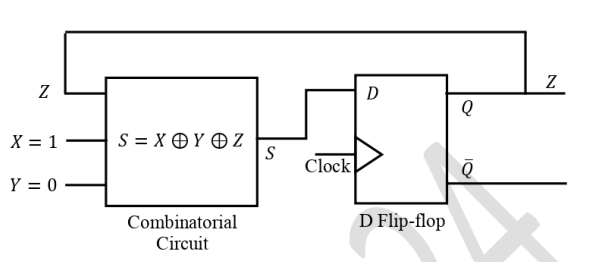
\includegraphics[width=0.6\columnwidth]{Figures/q25.png}
        \caption{}
    \end{figure}
    \begin{enumerate}
        \begin{multicols}{2}
            \item $S=0, Z=0$
            \item $S=0, Z=1$
            \item $S=1, Z=0$
            \item $S=1, Z=1$
        \end{multicols}
    \end{enumerate}

    \hfill{\brak{\text{GATE EE 2024}}}

    \item To obtain the Boolean function $F\brak{X,Y} = \overline{X}Y + X\overline{Y}$, the inputs $PQRS$ in the figure should be
    \begin{figure}[H]
        \centering
        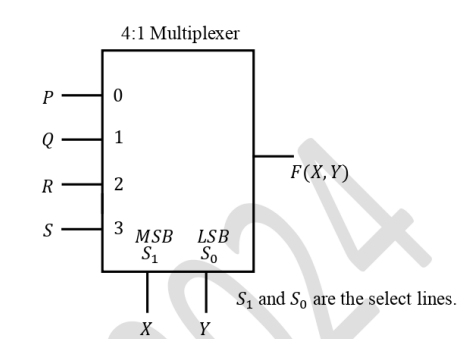
\includegraphics[width=0.5\columnwidth]{Figures/q26.png}
        \caption{}
    \end{figure}
    \begin{enumerate}
        \begin{multicols}{4}
            \item $1010$
            \item $1110$
            \item $0110$
            \item $0001$
        \end{multicols}
    \end{enumerate}

    \hfill{\brak{\text{GATE EE 2024}}}

    \item If the following switching devices have similar power ratings, which one of them is the fastest?
    \begin{enumerate}
        \begin{multicols}{4}
            \item SCR
            \item GTO
            \item IGBT
            \item Power MOSFET
        \end{multicols}
    \end{enumerate}

    \hfill{\brak{\text{GATE EE 2024}}}

    \item A single-phase triac based AC voltage controller feeds a series RL load. The input AC supply is $230$ V, $50$ Hz. The values of $R$ and $L$ are $10$ $\ohm$ and $18.37$ mH, respectively. The minimum triggering angle of the triac to obtain controllable output voltage is
    \begin{enumerate}
        \begin{multicols}{4}
            \item $15\degree$
            \item $30\degree$
            \item $45\degree$
            \item $60\degree$
        \end{multicols}
    \end{enumerate}

    \hfill{\brak{\text{GATE EE 2024}}}

    \item Let $X$ be a discrete random variable that is uniformly distributed over the set $\{-10, -9, \dots, 0, \dots, +9, 10\}$. Which of the following random variables is/are uniformly distributed?
    \begin{enumerate}
        \begin{multicols}{2}
            \item $X^2$
            \item $X^3$
            \item $\brak{X-5}^2$
            \item $\brak{X+10}^2$
        \end{multicols}
    \end{enumerate}

    \hfill{\brak{\text{GATE EE 2024}}}

    \item Which of the following complex functions is/are analytic on the complex plane?
    \begin{enumerate}
        \item $f\brak{z} = j\text{Re}\brak{z}$
        \item $f\brak{z} = \text{Im}\brak{z}$
        \item $f\brak{z} = e^{\text{Re}\brak{z}}$
        \item $f\brak{z} = z^2 - z$
    \end{enumerate}

    \hfill{\brak{\text{GATE EE 2024}}}

    \item Consider the complex function $f(z) = \cos(z) + e^{z^2}$. The coefficient of $z^2$ in the Taylor series expansion of $f(z)$ about the origin is \underline{\hspace{2cm}} \brak{\text{rounded off to 1 decimal place}}.

    \hfill{\brak{\text{GATE EE 2024}}}

    \item The sum of the eigenvalues of the matrix $A = \myvec{2 & 1 \\ 1 & 2}$ is \underline{\hspace{2cm}} \brak{\text{rounded off to the nearest integer}}.

    \hfill{\brak{\text{GATE EE 2024}}}

    \item Let $X(\omega)$ be the Fourier transform of the signal $x(t) = e^{-\abs{t}}\cos(t)$, $-\infty < t < \infty$. The value of the derivative of $X(\omega)$ at $\omega=0$ is \underline{\hspace{2cm}} \brak{\text{rounded off to 1 decimal place}}.

    \hfill{\brak{\text{GATE EE 2024}}}

    \item The incremental cost curves of two generators \brak{\text{Gen A and Gen B}} in a plant supplying a common load are shown in the figure. If the incremental cost of supplying the common load is Rs. $7400$ per MWh, then the common load in MW is \underline{\hspace{2cm}} \brak{\text{rounded off to the nearest integer}}.
    \begin{figure}[H]
        \centering
        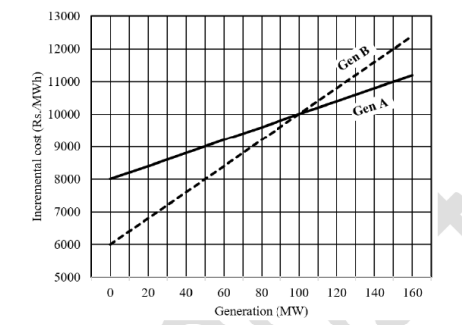
\includegraphics[width=0.6\columnwidth]{q34}
        \caption{}
    \end{figure}

    \hfill{\brak{\text{GATE EE 2024}}}

    \item  A forced commutated thyristorized step-down chopper is shown in the figure.
Neglect the ON-state drop across the power devices. Assume that the capacitor is
initially charged to 50 V with the polarity shown in the figure. The load current $I_l$
can be assumed to be constant at 10 A. Initially, Thy is ON and Thy is OFF. The
turn-off time available to $Th_M$ in microseconds, when $Th_A$ is triggered, is
(rounded off to the nearest integer)..
    \begin{figure}[H]
        \centering
        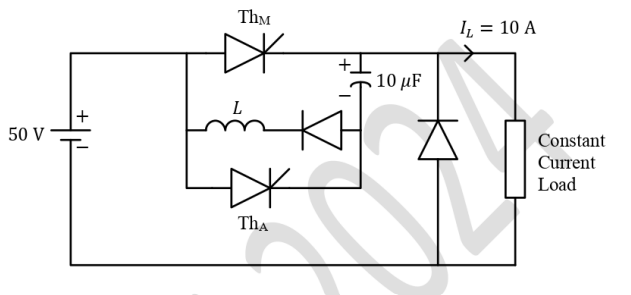
\includegraphics[width=0.5\columnwidth]{q35}
        \caption{}
    \end{figure}

    \hfill{\brak{\text{GATE EE 2024}}}

     \item Consider a vector $\bar{u} = 2\hat{x} + \hat{y} + 2\hat{z}$, where $\hat{x}, \hat{y}, \hat{z}$ represent unit vectors along the coordinate axes $x, y, z$ respectively. The directional derivative of the function $f\brak{x, y, z} = 2\ln\brak{xy} + \ln\brak{yz} + 3\ln\brak{xz}$ at the point $\brak{x, y, z} = \brak{1, 1, 1}$ in the direction of $\bar{u}$ is
    \begin{enumerate}
        \item $0$
        \item $\frac{7}{5\sqrt{2}}$
        \item $7$
        \item $21$
    \end{enumerate}


    \hfill{\brak{\text{GATE EE 2024}}}

    \item The input $x\brak{t}$ and the output $y\brak{t}$ of a system are related as
    \begin{align*}
        y\brak{t} = e^{-t} \int_{-\infty}^{t} e^{\tau} x\brak{\tau} d\tau, \quad -\infty < t < \infty.
    \end{align*}
    The system is
    \begin{enumerate}
        \item nonlinear.
        \item linear and time-invariant.
        \item linear but not time-invariant.
        \item noncausal.
    \end{enumerate}
    \hfill{\brak{\text{GATE EE 2024}}}

    \item Consider the discrete-time systems $T_1$ and $T_2$ defined as follows:
    \begin{align*}
        \{T_1x\}[n] &= x[0] + x[1] + \dots + x[n] \\
        \{T_2x\}[n] &= x[0] + \frac{1}{2}x[1] + \dots + \frac{1}{2^n}x[n]
    \end{align*}
    Which one of the following statements is true?
    \begin{enumerate}
        \item $T_1$ and $T_2$ are BIBO stable.
        \item $T_1$ and $T_2$ are not BIBO stable.
        \item $T_1$ is BIBO stable but $T_2$ is not BIBO stable.
        \item $T_1$ is not BIBO stable but $T_2$ is BIBO stable.
    \end{enumerate}

    \hfill{\brak{\text{GATE EE 2024}}}

     \item A 3-phase, $11$ kV, $10$ MVA synchronous generator is connected to an inductive load of power factor $\brak{\sqrt{3}/2}$ via a lossless line with a per-phase inductive reactance of $5 \ohm$. The per-phase synchronous reactance of the generator is $30 \ohm$ with negligible armature resistance. If the generator is producing the rated current at the rated voltage, then the power factor at the terminal of the generator is
    \begin{enumerate}
        \begin{multicols}{2}
            \item $0.63$ lagging.
            \item $0.87$ lagging.
            \item $0.63$ leading.
            \item $0.87$ leading.
        \end{multicols}
    \end{enumerate}

    \hfill{\brak{\text{GATE EE 2024}}}

     \item If the Z-transform of a finite-duration discrete-time signal $x[n]$ is $X\brak{z}$, then the Z-transform of the signal $y[n] = x[2n]$ is
    \begin{enumerate}
        \item $Y\brak{z} = X\brak{z^2}$
        \item $Y\brak{z} = \frac{1}{2}[X\brak{z^{-1/2}} + X\brak{-z^{-1/2}}]$
        \item $Y\brak{z} = \frac{1}{2}[X\brak{z^{1/2}} + X\brak{-z^{1/2}}]$
        \item $Y\brak{z} = \frac{1}{2}[X\brak{z^2} + X\brak{-z^2}]$
    \end{enumerate}

    \hfill{\brak{\text{GATE EE 2024}}}

    \item For the three-bus lossless power network shown in the figure, the voltage magnitudes at all the buses are equal to $1$ per unit \brak{pu}, and the differences of the voltage phase angles are very small. The line reactances are marked in the figure, where $\alpha, \beta, \gamma,$ and $x$ are strictly positive. The bus injections $P_1$ and $P_2$ are in pu. If $P_1 = mP_2$, where $m > 0$, and the real power flow from bus 1 to bus 2 is $0$ pu, then which one of the following options is correct?
    \begin{figure}[H]
        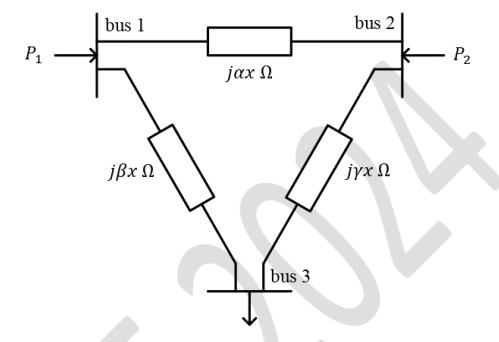
\includegraphics[width=0.6\columnwidth]{Figures/q41.png}
        \centering
        \caption{}
    \end{figure}
    \begin{enumerate}
        \item $\gamma = m\beta$
        \item $\beta = m\gamma$
        \item $\alpha = m\gamma$
        \item $\alpha = m\beta$
    \end{enumerate}

    \hfill{\brak{\text{GATE EE 2024}}}

     \item A BJT biasing circuit is shown in the figure, where $V_{BE} = 0.7$ V and $\beta = 100$. The Quiescent Point values of $V_{CE}$ and $I_C$ are respectively
    \begin{figure}[H]
        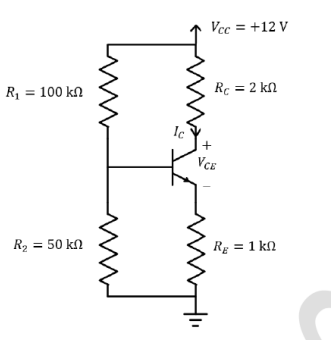
\includegraphics[width=0.5\columnwidth]{Figures/q42.png}
        \centering
        \caption{}
    \end{figure}
    \begin{enumerate}
        \begin{multicols}{2}
            \item $4.6$ V and $2.46$ mA
            \item $3.5$ V and $2.46$ mA
            \item $2.61$ V and $3.13$ mA
            \item $4.6$ V and $3.13$ mA
        \end{multicols}
    \end{enumerate}

    \hfill{\brak{\text{GATE EE 2024}}}

    \item Let $f\brak{t}$ be a real-valued function whose second derivative is positive for $-\infty < t < \infty$. Which of the following statements is/are always true?
    \begin{enumerate}
        \item $f\brak{t}$ has at least one local minimum.
        \item $f\brak{t}$ cannot have two distinct local minima.
        \item $f\brak{t}$ has at least one local maximum.
        \item The minimum value of $f\brak{t}$ cannot be negative.
    \end{enumerate}
    \hfill{\brak{\text{GATE EE 2024}}}

    \item Consider the function $f\brak{t} = \brak{\max\brak{0, t}}^2$ for $-\infty < t < \infty$, where $\max\brak{a, b}$ denotes the maximum of $a$ and $b$. Which of the following statements is/are true?
    \begin{enumerate}
        \item $f\brak{t}$ is not differentiable.
        \item $f\brak{t}$ is differentiable and its derivative is continuous.
        \item $f\brak{t}$ is differentiable but its derivative is not continuous.
        \item $f\brak{t}$ and its derivative are differentiable.
    \end{enumerate}

    \hfill{\brak{\text{GATE EE 2024}}}

   \item Which of the following differential equations is/are nonlinear?
    \begin{enumerate}
        \item $t x\brak{t} + \frac{dx\brak{t}}{dt} = t^2e^t, \quad x\brak{0} = 0$
        \item $\frac{1}{2}e^t + x\brak{t} + \frac{dx\brak{t}}{dt} = 0, \quad x\brak{0} = 0$
        \item $x\brak{t}\cos t - \frac{dx\brak{t}}{dt}\sin t = 1, \quad x\brak{0} = 0$
        \item $x\brak{t} + e^{\brak{\frac{dx\brak{t}}{dt}}} = 1, \quad x\brak{0} = 0$
    \end{enumerate}
    \hfill{\brak{\text{GATE EE 2024}}}

    \item For a two-phase network, the phase voltages $V_p$ and $V_q$ are to be expressed in terms of sequence voltages $V_\alpha$ and $V_\beta$ as $\myvec{V_p \\ V_q} = S \myvec{V_\alpha \\ V_\beta}$. The possible option\brak{s} for matrix S is/are
    \begin{enumerate}
        \item $\myvec{1 & 1 \\ 1 & -1}$
        \item $\myvec{1 & 1 \\ 1 & 1}$
        \item $\myvec{1 & 1 \\ 1 & 0}$
        \item $\myvec{-1 & 1 \\ 1 & 1}$
    \end{enumerate}


    \hfill{\brak{\text{GATE EE 2024}}}

    \item Which of the following options is/are correct for the Automatic Generation Control \brak{AGC} and Automatic Voltage Regulator \brak{AVR} installed with synchronous generators?
    \begin{enumerate}
        \item AGC response has a local effect on frequency while AVR response has a global effect on voltage.
        \item AGC response has a global effect on frequency while AVR response has a local effect on voltage.
        \item AGC regulates the field current of the synchronous generator while AVR regulates the generator's mechanical power input.
        \item AGC regulates the generator's mechanical power input while AVR regulates the field current of the synchronous generator.
    \end{enumerate}

    \hfill{\brak{\text{GATE EE 2024}}}

    \item Two passive two-port networks P and Q are connected as shown in the figure. The impedance matrix of network P is $Z_P = \myvec{40 & 60 \\ 80 & 100} \ohm$. The admittance matrix of network Q is $Y_Q = \myvec{5 & -2.5 \\ -2.5 & 1}$ S. Let the ABCD matrix of the two-port network R in the figure be $\myvec{\alpha & \beta \\ \gamma & \delta}$. The value of $\beta$ in $\ohm$ is \underline{\hspace{2cm}} \brak{\text{rounded off to 2 decimal places}}.
    \begin{figure}[H]
        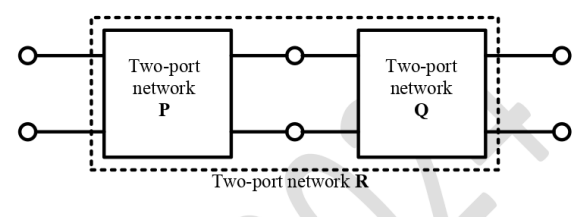
\includegraphics[width=0.7\columnwidth]{Figures/q48.png}
        \centering
        \caption{}
    \end{figure}

    \hfill{\brak{\text{GATE EE 2024}}}

    \item For the circuit shown in the figure, the source frequency is $5000$ rad/sec. The mutual inductance between the magnetically coupled inductors is $5$ mH with their self inductances being $125$ mH and $1$ mH. The Thevenin's impedance, $Z_{th}$, between the terminals P and Q in $\ohm$ is \underline{\hspace{2cm}} \brak{\text{rounded off to 2 decimal places}}.
    \begin{figure}[H]
        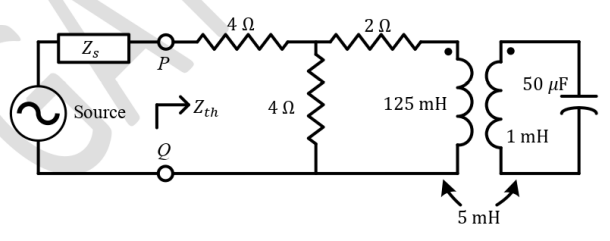
\includegraphics[width=0.8\columnwidth]{Figures/q49.png}
        \centering
        \caption{}
    \end{figure}
    \hfill{\brak{\text{GATE EE 2024}}}

    \item In the circuit shown, $Z_1 = 50\angle-90^\degree \ohm$ and $Z_2 = 200\angle-30^\degree \ohm$. It is supplied by a three phase 400 V source with the phase sequence being R-Y-B. Assume the watt meters $W_1$ and $W_2$ to be ideal. The magnitude of the difference between the readings of $W_1$ and $W_2$ in watts is \underline{\hspace{2cm}} \brak{\text{rounded off to 2 decimal places}}.
    \begin{figure}[H]
        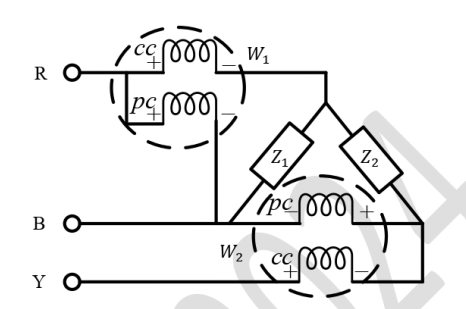
\includegraphics[width=0.6\columnwidth]{Figures/q50.png}
        \centering
        \caption{}
    \end{figure}

    \hfill{\brak{\text{GATE EE 2024}}}

    \item In the $\brak{x, y, z}$ coordinate system, three point-charges $Q, Q,$ and $aQ$ are located in free space at $\brak{-1, 0, 0}, \brak{1, 0, 0},$ and $\brak{0, -1, 0}$, respectively. The value of $\alpha$ for the electric field to be zero at $\brak{0, 0.5, 0}$ is \underline{\hspace{2cm}} \brak{\text{rounded off to 1 decimal place}}.

    \hfill{\brak{\text{GATE EE 2024}}}

    \item The given equation represents a magnetic field strength $\vec{H}\brak{r, \theta, \phi}$ in the spherical coordinate system, in free space. Here, $\hat{r}$ and $\hat{\theta}$ represent the unit vectors along $r$ and $\theta$, respectively. The value of $P$ in the equation should be \underline{\hspace{2cm}} \brak{\text{rounded off to the nearest integer}}.
    \begin{align*}
        \vec{H}\brak{r, \theta, \phi} = \frac{1}{r^3}\brak{\hat{r}P\cos\theta + \hat{\theta}\sin\theta}
    \end{align*}

    \hfill{\brak{\text{GATE EE 2024}}}

    \item If the energy of a continuous-time signal $x\brak{t}$ is $E$ and the energy of the signal $2x\brak{2t-1}$ is $cE$, then $c$ is \underline{\hspace{2cm}} \brak{\text{rounded off to 1 decimal place}}.

    \hfill{\brak{\text{GATE EE 2024}}}

    \item A 3-phase star connected slip ring induction motor has the following parameters referred to the stator: $R_s = 3 \ohm, X_s = 2 \ohm, R_r' = 2 \ohm, X_r' = 2.5 \ohm$. The per phase stator to rotor effective turns ratio is $3:1$. The rotor winding is also star connected. The magnetizing reactance and core loss of the motor can be neglected. To have maximum torque at starting, the value of the extra resistance in ohms \brak{\text{referred to the rotor side}} to be connected in series with each phase of the rotor winding is \underline{\hspace{2cm}} \brak{\text{rounded off to 2 decimal places}}.

    \hfill{\brak{\text{GATE EE 2024}}}

    \item A 5 kW, 220 V DC shunt motor has $0.5 \ohm$ armature resistance including brushes. The motor draws a no-load current of $3$ A. The field current is constant at $1$ A. Assuming that the core and rotational losses are constant and independent of the load, the current \brak{\text{in amperes}} drawn by the motor while delivering the rated load, for the best possible efficiency, is \underline{\hspace{2cm}} \brak{\text{rounded off to 2 decimal places}}.

    \hfill{\brak{\text{GATE EE 2024}}}

    \item The single line diagram of a lossless system is shown in the figure. The system is operating in steady-state at a stable equilibrium point with the power output of the generator being $P_{\max}\sin\delta$, where $\delta$ is the load angle and the mechanical power input is $0.5 P_{\max}$. A fault occurs on line 2 such that the power output of the generator is less than $0.5 P_{\max}$ during the fault. After the fault is cleared by opening line 2, the power output of the generator is $\brak{P_{\max}/\sqrt{2}}\sin\delta$. If the critical fault clearing angle is $\pi/2$ radians, the accelerating area on the power angle curve is \underline{\hspace{2cm}} times $P_{\max}$ \brak{\text{rounded off to 2 decimal places}}.
    \begin{figure}[H]
        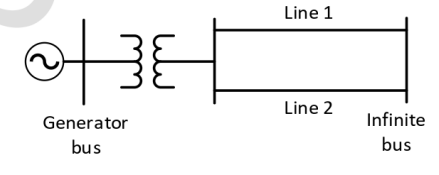
\includegraphics[width=0.6\columnwidth]{Figures/q56.png}
        \centering
        \caption{}
    \end{figure}

    \hfill{\brak{\text{GATE EE 2024}}}

    \item Consider the closed-loop system shown in the figure with
    \begin{align*}
        G\brak{s} = \frac{K\brak{s^2 - 2s + 2}}{\brak{s^2 + 2s + 5}}.
    \end{align*}
    The root locus for the closed-loop system is to be drawn for $0 \le K < \infty$. The angle of departure \brak{\text{between $0^\degree$ and $360^\degree$}} of the root locus branch drawn from the pole $\brak{-1+j2}$, in degrees, is \underline{\hspace{2cm}} \brak{\text{rounded off to the nearest integer}}.
    \begin{figure}[H]
        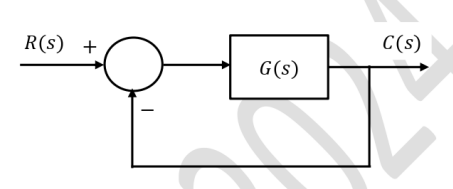
\includegraphics[width=0.6\columnwidth]{Figures/q57.png}
        \centering
        \caption{}
    \end{figure}

    \hfill{\brak{\text{GATE EE 2024}}}

    \item Consider the stable closed-loop system shown in the figure. The asymptotic Bode magnitude plot of $G\brak{s}$ has a constant slope of $-20$ dB/decade at least till $100$ rad/sec with the gain crossover frequency being $10$ rad/sec. The asymptotic Bode phase plot remains constant at $-90^\degree$ at least till $\omega = 10$ rad/sec. The steady-state error of the closed-loop system for a unit ramp input is \underline{\hspace{2cm}} \brak{\text{rounded off to 2 decimal places}}.
    \begin{figure}[H]
        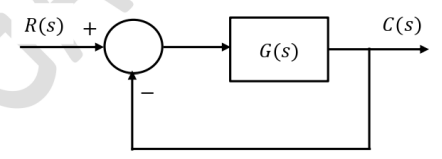
\includegraphics[width=0.6\columnwidth]{Figures/q58.png}
        \centering
        \caption{}
    \end{figure}

    \hfill{\brak{\text{GATE EE 2024}}}
\item Consider the stable closed-loop system shown in the figure. The magnitude and phase values of the frequency response of $G\brak{s}$ are given in the table. The value of the gain $K_I \brak{>0}$ for a $50^\degree$ phase margin is \underline{\hspace{2cm}} \brak{\text{rounded off to 2 decimal places}}.
    \begin{table}[H]
        \centering
        \caption*{}
        \label{tab:freqresp}
        \begin{tabular}{|c|c|c|}
            \hline
            $\omega$ in rad/sec & Magnitude in dB & Phase in degrees \\
            \hline
            $0.5$ & $-7$ & $-40$ \\
            $1.0$ & $-10$ & $-80$ \\
            $2.0$ & $-18$ & $-130$ \\
            $10.0$ & $-40$ & $-200$ \\
            \hline
        \end{tabular}
    \end{table}
    \begin{figure}[H]
        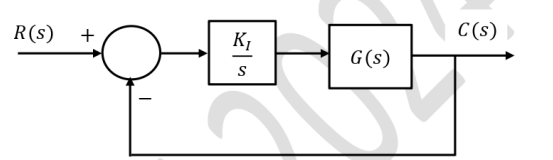
\includegraphics[width=0.7\columnwidth]{Figures/q59.png}
        \centering
        \caption{}
    \end{figure}

    \hfill{\brak{\text{GATE EE 2024}}}

    \item In the given circuit, the diodes are ideal. The current $I$ through the diode $D1$ in milliamperes is \underline{\hspace{2cm}} \brak{\text{rounded off to two decimal places}}.
    \begin{figure}[H]
        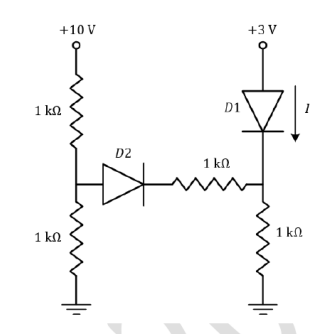
\includegraphics[width=0.6\columnwidth]{Figures/q60.png}
        \centering
        \caption{}
    \end{figure}

    \hfill{\brak{\text{GATE EE 2024}}}
    \item A difference amplifier is shown in the figure. Assume the op-amp to be ideal. The CMRR \brak{\text{in dB}} of the difference amplifier is \underline{\hspace{2cm}} \brak{\text{rounded off to 2 decimal places}}.
    \begin{figure}[H]
        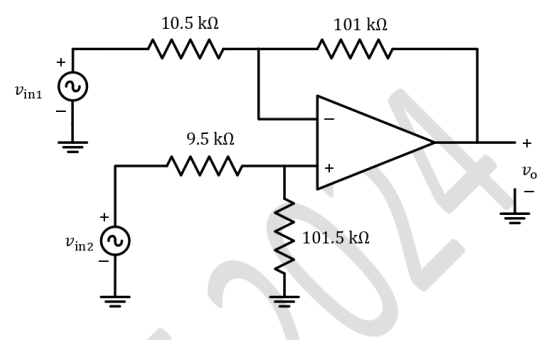
\includegraphics[width=0.8\columnwidth]{Figures/q61.png}
        \centering
        \caption{}
    \end{figure}

    \hfill{\brak{\text{GATE EE 2024}}}

    \item A single-phase half-controlled bridge converter supplies an inductive load with ripple free load current. The triggering angle of the converter is $60^\degree$. The ratio of the rms value of the fundamental component of the input current to the rms value of the total input current of the bridge is \underline{\hspace{2cm}} \brak{\text{rounded off to 3 decimal places}}.

    \hfill{\brak{\text{GATE EE 2024}}}

    \item A single-phase full bridge voltage source inverter \brak{VSI} feeds a purely inductive load. The inverter output voltage is a square wave in $180^\degree$ conduction mode. The fundamental frequency of the output voltage is $50$ Hz. If the DC input voltage of the inverter is $100$ V and the value of the load inductance is $20$ mH, the peak-to-peak load current in amperes is \underline{\hspace{2cm}} \brak{\text{rounded off to the nearest integer}}.

    \hfill{\brak{\text{GATE EE 2024}}}
\item In the DC-DC converter shown in the figure, the current through the inductor is continuous. The switching frequency is $500$ Hz. The voltage $\brak{V_o}$ across the load is assumed to be constant and ripple free. The peak inductor current in amperes is \underline{\hspace{2cm}} \brak{\text{rounded off to the nearest integer}}.
    \begin{figure}[H]
        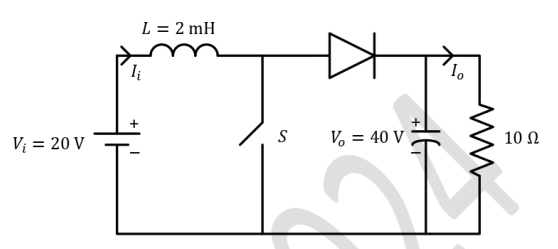
\includegraphics[width=0.8\columnwidth]{Figures/q64.png}
        \centering
        \caption{}
    \end{figure}

    \hfill{\brak{\text{GATE EE 2024}}}

    \item A single-phase full-controlled thyristor converter bridge is used for regenerative braking of a separately excited DC motor with the following specifications:
    \begin{table}[H]
        \centering
        \caption*{}
        \label{tab:motor_specs}
        \begin{tabular}{|l|l|}
            \hline
            Rated armature voltage & $210$ V \\
            Rated armature current & $10$ A \\
            Rated speed & $1200$ rpm \\
            Armature resistance & $1 \ohm$ \\
            Input to the converter bridge & $240$ V at $50$ Hz \\
            \hline
        \end{tabular}
    \end{table}
    The armature of the DC motor is fed from the full-controlled bridge and the field current is kept constant.
    Assume that the motor is running at $600$ rpm and the armature terminals of the motor are suitably reversed for regenerative braking. If the armature current of the motor is to be maintained at the rated value, the triggering angle of the converter bridge in degrees should be \underline{\hspace{2cm}} \brak{\text{rounded off to 2 decimal places}}.

    \hfill{\brak{\text{GATE EE 2024}}}
\end{enumerate}
\end{document}
